% !TEX root = ../main.tex

% \pagenumbering{arabic}
% \setcounter{page}{1}


\chapter{Background} \label{sec:background}

In this chapter, we go over the building blocks for blockchain technology and other concepts required for understanding this dissertation.

\section{Blockchain}
A technical challenge in developing a decentralized network has been establishing a consensus mechanism (See section~\ref{consensus_mechanism}) that operates without centralized trust among participants. "Trust" here refers to the reliance on a central authority to validate transactions, a notion Bitcoin managed to eliminate. Implementing an online ledger on a single computer is straightforward, involving a database with public read access and restricted write access controlled by a central authority. This setup inherently trusts the central party managing the server. However, as soon as you begin to have more computers in the decentralized network, the question arises, how to keep updating the database and enforce honesty amongst the network participants? Prior to Bitcoin, attempts to decentralize this model were made starting in the 1980's~\cite{narayanan2017bitcoin}, but it wasn't until Nakamoto's work in 2008~\cite{nakamoto2008bitcoin} that a viable solution emerged, leveraging a network of nodes incentivized to maintain and validate a public ledger without a central authority. A decentralized network here means that no single entity controls the network, and the network is open to anyone to join or leave at any time.

A (full) node in the Bitcoin network, is a computer that maintains a copy of the blockchain and is verifying transactions and blocks. Nodes that are configured to create new blocks, called a miner, are rewarded with new cryptocurrency (bitcoin) for their efforts in transaction verification and block formation (further explained in~\ref{pow}). Transactions, essentially value transfers, are the fundamental components of the blockchain. The blockchain is a list of such transactions grouped into sequential blocks (explained in more details in~\ref{block_creation}). The order within these blocks is critical, indicating the sequence of transactions across the network (See Chapter~\ref{sec:frontrunning}). 


Public blockchains are a promising underlying technology for many applications. Their aim of providing decentralization, transparency, and immutability correlates with the security goals of many use-cases. However, blockchains are also slow, expensive, and have practical limits to their functionality. I predict they can and will replace many intermediary entities we know of today. There is a gap in the mental model of what people (industry and academia) think blockchain provides and what it actually does~\cite{RKYCC20}. Even developers need to change many assumptions given the public aspect of how a blockchain works, and system designers have to rethink the data flow within their applications. We hope to illustrate this throughout the dissertation. 


\begin{figure}[t]
    \centering
     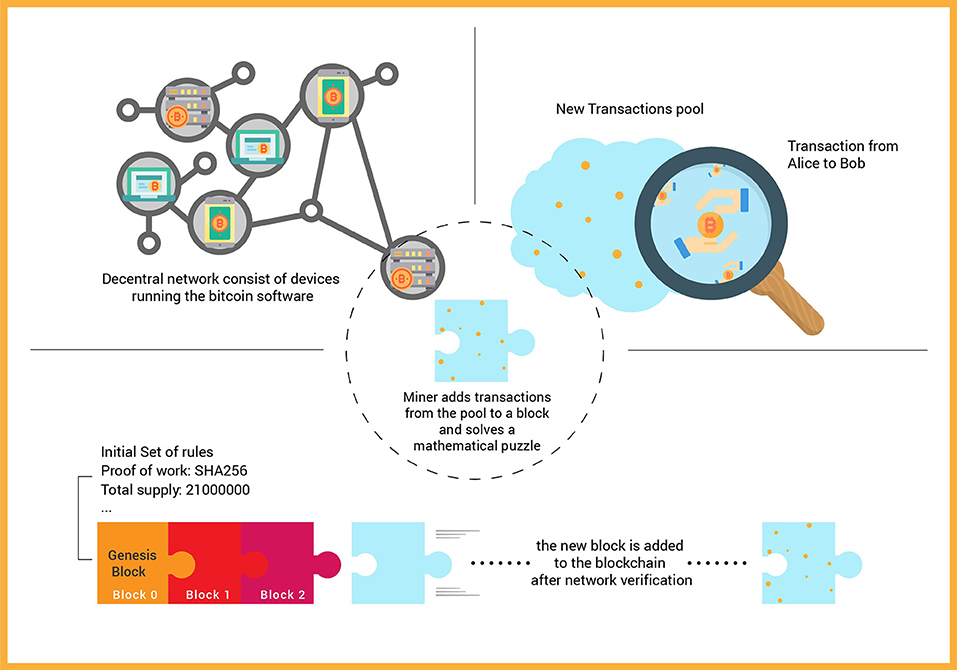
\includegraphics[width=0.9\textwidth]{figures/blockchain-buildingblocks.jpg}
    \caption[The Building Blocks of Blockchain Technology]{The building blocks of blockchain technology} 
\end{figure}


This technology has the potential of many interesting applications, from financial use cases (\eg Bitcoin~\cite{nakamoto2008bitcoin}), asset trading and markets~\cite{clark2014decentralizing,uniswapexplained}, insurance and futures~\cite{massacci2018futuresmex,muller2000weather}, tamper-resistant record storage~\cite{catenaEth}, and online voting~\cite{mccorry2017smart,aragonwebsite}. Bitcoin, started in 2009, was the first application of blockchain technology and since then the concept of decentralized ledger has grown to many other applications that just a ledger holding transaction data.


Bitcoin pioneered the use of a decentralized ledger for tracking cryptocurrency transactions. However, its limitations prompted the development of other blockchain technologies seeking to enhance its original model. Ethereum, introduced by Vitalik Buterin, expanded on Bitcoin’s capabilities by incorporating smart contracts, allowing for complex, programmable transactions beyond simple value transfers~\cite{buterin2014next}. This added functionality, however, comes at the cost of speed and efficiency, with Ethereum facing scalability challenges. To address these, developers are exploring solutions such as layer 2 protocols~\cite{clark2018sok:online,optimismgithub,kalodner2018arbitrum}, which operate on top of the Ethereum blockchain to increase transaction speeds and reduce costs.

In parallel, privacy-focused cryptocurrencies like Monero~\cite{monero} and Zcash~\cite{hopwood2016zcash} have been developed to address another limitation of Bitcoin: privacy. These platforms implement advanced cryptographic techniques to offer enhanced privacy and anonymity for users, making transaction details and participant identities obscure~\cite{van2013cryptonote, miers2013zerocoin}. Monero, for example, uses ring signatures and stealth addresses to protect user privacy~\cite{cryptoeprint2015}, distinguishing itself from Bitcoin's transparent transaction ledger. It should be noted that these privacy features are not perfect yet and have been found vulnerable in the past~\cite{kumar2017traceability,miller2017empirical}.



\subsection{Consensus Mechanism}\label{consensus_mechanism}
A consensus mechanism is a fundamental protocol within blockchain technology that enables network participants, often referred to as validators, to agree on the state of the ledger, despite the absence of anyone coordinating their actions or them trusting each other fully. It is the bedrock of blockchain's reliability and security, ensuring that each participant has a consistent view of the transaction record (final state of the blockchain). This mechanism is crucial in decentralized systems like Bitcoin and Ethereum, where no central authority confirms the validity of transactions, or dictates who can play the role of a validator in the system. 

In essence, a consensus mechanism involves a series of processes and rules that nodes follow to validate new transactions, add them to the blockchain, and achieve agreement on the current state of the ledger. If all nodes are malicious, consensus is impossible; however protocols assume that at all times, a threshold (\eg 50\%; although the exact number and nature varies) of honest nodes will follow these processes and rules. These processes are designed to prevent fraudulent activities and to mitigate the influence of any single entity over the network. The most widely recognized consensus mechanisms are based on proof of work (PoW) and proof of stake (PoS).

\subsubsection{Proof of Work (PoW)} \label{pow}

Employed initially by Bitcoin and Ethereum, PoW requires nodes, called \textit{miners}, to solve cryptographic puzzles. Miners must solve the puzzle before being able to add a new block of transactions to the blockchain. This method, while robust in maintaining network security, is often criticized for its high energy consumption. In order to understand PoW a few cryptography primitives and other building blocks need to be explained.


\paragraph{Hash Functions.}
A hash function is a deterministic algorithm that takes an input (or 'message') and returns a fixed-size string of bytes, typically a digest that appears random. The output, known as the \textit{hash value} or the hash, is unique to each unique input: even a minor change in the input results in a significantly different output. This property, called the avalanche effect~\cite{feistel1973cryptography}, is crucial for security. Another important property of hash functions in the context of blockchain is \textit{collision resistance}, which ensures that it is highly improbable for two different inputs to produce the same output hash. This attribute is vital for maintaining the integrity of the blockchain, as it helps prevent tampering by ensuring that each block can be uniquely identified and verified through its hash. Hash functions are used for various purposes in blockchain, including generating addresses, creating digital fingerprints of data, and linking each block to the previous blocks in the blockchain securely. The nature of hash functions makes them one-way operations---while it's feasible to generate a hash from a given piece of data, it's computationally infeasible to reconstruct the original data from the hash. This one-way property, coupled with collision resistance, is crucial for blockchain security and digital signatures, as it prevents malicious actors from tampering with the data by making it exceedingly difficult to alter the data without detection.

%TODO: maybe add precise with notation. Like saying H(prevBlock, merkleRoot, nonce) ... 

\paragraph{Digital Signature.}\label{digital_signature}
Before delving into the operations of digital signatures, it's crucial to understand the context of Public Key Infrastructure (PKI)~\cite{adams1999understanding}, which underpins the security of digital signatures. PKI is a framework that describes encryption keys, including the creation, distribution, and verification of public and private keys. In this system, each user has a pair of keys: a public key and a private key. The public key is derived from the private key through cryptographic hash functions, ensuring that both keys are interconnected. The private key must be kept secure by the owner, as it is used to create digital signatures and blockchain transactions. Furthermore, the public key can be shared with anyone and is used to verify the authenticity of the message signed with the corresponding private key.

Digital signatures are a cryptographic tool used to ensure authenticity and integrity in digital communications and transactions. They function as a digital equivalent of a handwritten signature or stamped seal, providing enhanced security. This mechanism is pivotal for securing transactions on a blockchain. A digital signature process encompasses two main operations: signing and verifying. The signing operation involves generating a signature where an individual utilizes their private key to sign a message (or transaction) using a specific signature algorithm. This signature, once generated, is appended to the message and forwarded to the recipient. The verification process is initiated by the recipient, who employs the corresponding public key to apply a verification algorithm to the signature. A valid signature confirms that the message remains unchanged and authenticates that it was signed by the private key holder. This verification process is integral to blockchain transactions, safeguarding against tampering and ensuring transactions are legitimately conducted by the true owners of the digital assets.




\textblue{Add transactions as a building block. What they are. How they work relevative to public keys. How they are signed. What bad thing happens if your key is stolen. That kind of thing. This is relevant later for internal controls chapter.}

\textblue{Add mempool as well. Describe how a transaction is gossiped, how miners gather them in a mempool, how ordering is arbitrary (I know this was mentioned already but do it again here), how a block is put together, different miners will have different blocks, then go into mining.}

\paragraph{Mining.}

During the mining process, miners compete to solve a cryptographic puzzle, which involves finding a hash that meets a specific condition set by the network, typically an output value that is lower than a particular target (difficulty). This process requires miners to input data from the block header, which includes a reference to the previous block's hash---ensuring the integrity and continuity of the blockchain---and a set of signed transactions waiting in the mempool. Miners repeatedly hash this data with a varying nonce value until they find a valid hash that meets the network's difficulty criteria.

The first miner to solve the puzzle gets the privilege of adding the new block to the blockchain.\textblue{Soften this to match forking below} This block includes all the validated transactions, each verified through their digital signatures to ensure they are legitimate and authorized by the respective private key holders. The successful miner is then rewarded with newly minted cryptocurrency (like Bitcoin or Ether) and transaction fees from the transactions included in the block. This incentivization is crucial for encouraging participants to contribute their computational power to the network. The history of mining ecosystem is by itself an interesting story which some of it is discussed in ~\ref{sec:mininghistory}.

\textblue{Discuss forking, and re-orgs and how they resolve over time (you can borrow from page 131). Introduce idea of 0-confirmation, 1-confirmation, \etc (needed later). Describe hard fork vs soft fork. Describe what you need later for accounting section and things like bitcoin cash.}

\textblue{Discuss 51\% attack}

Mining is not just about creating new cryptocurrency units; it's the backbone of maintaining the decentralization, security, and integrity of the blockchain. By utilizing hash functions, it ensures that each block is securely linked to its predecessor, creating an immutable ledger. The reliance on digital signatures within each transaction enhances the security and authenticity of the transactions recorded in each block. The decentralized nature of mining, where multiple nodes compete to solve the puzzle, ensures that no single entity can control the network. This mechanism is the foundation of blockchain security.



\paragraph{Mining Pools.}
Mining pools exist particularly in networks that utilize the Proof of Work (PoW) consensus mechanism. They consist of groups of miners who combine their computational resources to increase their collective probability of successfully mining a block and receiving the rewards. Individual miners, especially those with limited hardware capabilities, might find it challenging to compete against more powerful, resource-rich miners. By joining a mining pool, these smaller miners effectively pool their hashing power, increasing their chances of solving the cryptographic puzzles required to add a block to the blockchain. When a pool successfully mines a block, the reward is distributed amongst its members in proportion to the computational power each contributed. This arrangement makes mining more accessible and potentially more profitable for individual miners, as it offers a more consistent and predictable return compared to solo mining, where rewards can be sporadic and significantly less frequent. Mining pools are instrumental in maintaining a degree of democratization in the mining process, ensuring that smaller players can still contribute to and benefit from the blockchain network. That being said, if a mining pool becomes too large, it can potentially control the network, leading to centralization and security concerns. We discuss more relevant details on mining pools in Chapter~\ref{sec:cryptojackingasic}.



\subsubsection{Proof of Stake (PoS).}
Proof of Stake is a system that relies on validators who ``stake'' their cryptocurrency holdings as collateral to participate in the process of managing the blockchain. Unlike Proof of Work (PoW), which requires energy-intensive computational work, PoS selects validators based on the amount of their staked cryptocurrency, creating a more energy-efficient process.

In PoS, the likelihood of a validator being chosen to propose or validate a block correlates with the size of their stake. Validators lock up a certain amount of cryptocurrency (32 ETH in Ethereum per validator), demonstrating their commitment to the network. This stake acts as a security deposit; validators who act against the network's rules or try to approve fraudulent transactions can lose part of their stake as a penalty, called slashing. This incentivizes good behaviour and secures the network. There are more actors in PoS comparing to PoW process \textblue{why?}.

In the PoS process, a ~\textit{block proposer} is comparable to a miner in PoW. The network algorithm selects a validator to propose a new block based on their stake and other factors like random selection for fairness~\cite{ethereumrandao}. The proposer's role is to gather transactions from the transaction pool (mempool), form them into a block, and propose it to the network. This block includes transaction data and a cryptographic hash of the previous block, maintaining the blockchain's integrity. The validator will receive a reward for proposing a block, which is typically a portion of the transaction fees included in the block and newly minted coins (ETH in the case of Ethereum).

The ~\textit{block builder} is a role often seen in more advanced PoS systems. They are responsible for constructing the block---organizing and prioritizing transactions. In some systems, this role is separated from the block proposer to introduce another layer of decentralization and efficiency. By decoupling block construction from proposal, it allows for more specialized handling of transaction inclusion, potentially leading to optimized transaction throughput and fee market dynamics. Block builders are currently used as part of the MEV mechanism, which is explained more in~\ref{MEVfrontrunning}. More over, a proposal to separate the block proposer and builder in Ethereum PoS is under consideration~\cite{ethereumPBS}.

~\textit{Relayers} are participants in the network who help in relaying information between different parties or layers. In the context of PoS, they might be involved in transmitting block proposals, transactions, or validation results. Relayers play a crucial role in ensuring the smooth flow of information across the network, which is vital for maintaining the blockchain's speed and reliability. Currently, relayers are mainly used between the block proposers and builders in MEV infrastructure.

In summary, in a PoS system, validators stake cryptocurrency to participate in the process of block creation and validation. The block proposer and builder work together to form and optimize new blocks, while relayers facilitate communication within the network. This system aims to offer a more energy-efficient and potentially more decentralized alternative to PoW.




\section{Ethereum}

Ethereum~\cite{wood2014ethereum} is a prominent public blockchain that has attracted the largest developer headcount compared to other blockchains. It is an extension of its predecessor, Bitcoin~\cite{nakamoto2008bitcoin}, but with significant enhancements, notably the addition of verbose \textit{smart contracts}. These smart contracts are applications residing on the blockchain that can immutably execute their verified code \textblue{what does verified code mean?}. Ethereum operates on a Turing-complete virtual machine, the \texttt{Ethereum Virtual Machine (EVM)}, allowing programs to live and be executed on the blockchain. This differs from Bitcoin's UTXO\footnote{Unspend Transaction Output} model, which primarily supports value transfers and has a scripting language for extending transaction functionality to a limited extent. In contrast, Ethereum's Turing-complete language opens up limitless possibilities.  All transactions and executions on Ethereum are verified by a decentralized network of nodes. The nodes are incentivized to verify transactions and execute smart contracts by receiving rewards in the form of Ether, the native cryptocurrency of Ethereum. 

Ethereum blockchain started in 2015 using the similar consensus mechanism as Bitcoin, called Proof of Work (PoW), also known as mining. However, in 2020, Ethereum started the transition to Proof of Stake (PoS) consensus mechanism. The main difference between PoW and PoS is that in PoW, the nodes are incentivized to solve a computationally hard puzzle to be able to add a block to the blockchain. However, in PoS, the nodes are incentivized to stake their Ether to be able to add a block to the blockchain. The PoS mechanism is more energy efficient and more scalable than PoW. Ethereum fully switched to PoS in September 2022 in an event called the \textit{Merge}, and reduced its energy consumption by 99.5\%~\cite{themerge}. In this dissertation, we do not directly focus on the consensus mechanisms, however, we will discuss the implications of the consensus mechanism on the blockchain security in chapter ~\ref{sec:frontrunning}. 


\subsection{Smart Contracts}

Smart contracts, a fundamental component of blockchain technology, particularly in the Ethereum ecosystem, represent a paradigm shift in how contractual agreements are executed and enforced. These contracts are essentially codebases that reside on the blockchain, acting as autonomous agents that carry out predefined functions when a user invokes the contract and certain conditions are met. 

At their core, Ethereum smart contracts are collections of code and data (state) residing at a specific address on the Ethereum blockchain. Developed primarily in Solidity, a high-level language specifically designed for Ethereum, these contracts encapsulate a set of rules and automatically enforce them through the code. Solidity, with its syntax similar to JavaScript and C++, enables developers to write applications that implement self-enforcing business logic encapsulated within smart contracts, thereby removing the need for intermediaries.

Smart contracts are compiled into bytecode and deployed on the Ethereum blockchain. Once deployed, they become immutable – their code cannot be altered, ensuring the integrity of the contract. Execution of a smart contract is triggered by transactions. These transactions are sent by external Ethereum accounts \textblue{define external}, containing the necessary information to invoke specific functions within the contract. Every operation in a smart contract requires a certain amount of \textit{gas}, a unit that measures the computational effort required to execute operations. Users initiating transactions must supply enough ether, Ethereum's native cryptocurrency, to cover the gas costs, which are determined by the complexity of the operations and the current network demand. This mechanism prevents inefficient or malicious contracts from wasting network resources. Smart contracts maintain an internal state stored on the blockchain. This state can include variables, balances, and other contract-specific data. When a contract's function is executed, it can alter its state (e.g., updating balances, changing ownership records) and can also interact with other contracts, thereby enabling complex decentralized applications (DApps).\textblue{I think you should explain gas more precisely, tied to OPCODES, you cannot always predict how much gas because it might change before your transaction runs, gas auctions and how they work, rough sense of cost in CAD, \etc. This is important for the front-running chapter.}

While Ethereum smart contracts offer a wide range of functionalities, they are not without limitations. Their capabilities extend from creating tokenized assets and managing digital identities to executing decentralized finance (DeFi) transactions and running complex DApps. Use cases like decentralized gambling platforms, voting systems, and automated payroll services exemplify their versatility. However, the ``unstoppable'' nature of these contracts also poses challenges, particularly in terms of security and scalability. The code's immutability means that any flaws or vulnerabilities in the contract cannot be easily rectified post-deployment, emphasizing the need for rigorous testing and auditing pre-deployment. Security in smart contracts is paramount, as vulnerabilities can lead to significant financial losses. Common issues include reentrancy attacks, where a malicious contract can repeatedly call a function in the original contract, and problems arising from visibility and access control, where private data or functions can be unintentionally exposed. 

As noted earlier, everything on a blockchain is compromised of transactions and blocks. The order of the transactions in each block indicates the order of events and smart contract executions in the Ethereum blockchain. Given that miners, and recently entities named \textit{block builders}, are in control of the order, it is possible for these entities to reorder the transaction in a block, or even not include a transaction in a block for higher financial gain from the new order. This is the basics of blockchain front-running that we discuss in the next chapters. 


\subsection{P2P Network}

The Ethereum network, envisioned as a global, decentralized computer, operates on a peer-to-peer (P2P) basis, a key feature that distinguishes it from traditional centralized systems. This P2P architecture is foundational to Ethereum's functionality, enabling a trustless and permissionless environment where anyone can participate in the network. In the core of the design principles of Ethereum's P2P network, there are three main concepts: decentralization, trustless interactions, and permissionless nature. These concepts are the foundation of the Ethereum network and are the main reasons for the success of Ethereum. More technical details on how the P2P network impacts the information flow is discussed in ~\ref{offChainInfrastructure}.

\paragraph{Decentralization and Accessibility:} Ethereum's network is designed to be fully decentralized, eliminating any central point of control or failure. This decentralization ensures that the network remains resilient against attacks and censorship. It is worthy to note that these are the ideal properties and the current state of the network does not have full resiliency against these attacks. The accessibility of the network allows anyone to run a full node, contributing to the network's health and security.

\paragraph{Trustless Interactions:} In Ethereum's P2P network, nodes interact without needing to trust each other. Trustlessness is achieved through cryptographic verification methods and consensus algorithms, ensuring that all transactions and blocks adhere to the network's rules without requiring mutual trust amongst participants.

\paragraph{Permissionless Nature:} The network's permissionless design means that anyone can join and leave the network at will, participate in mining activities, and contribute to the network's consensus process. This open-access principle is fundamental to Ethereum's ethos of inclusivity and decentralization.

As Ethereum has grown in popularity, the network has faced scalability issues, leading to congestion and high transaction fees. Many layer-2 scaling solutions like rollups, are being developed to address these challenges. 

\subsection{Transactions}

Transactions are the means by which users interact with the blockchain, initiating value transfers and executing smart contracts' functionalities. Transactions are cryptographically signed messages sent by externally owned accounts (EOA) to the network~\cite{transactionsethereumorg}, containing the necessary information to transfer value to the recipient or to invoke specific functions within the contract. Each transaction includes the sender's signature, recipient's address, the amount of Ether to be transferred, the gas limit and price, the data associated with the transaction (\eg the function to be called and the input arguments), and a nonce. The gas price is the amount of Ether the sender is willing to pay per unit of gas (up to the gas limit), which is determined by the complexity of the transaction and the current network demand~\cite{gasethereumorg}. Transactions are broadcast to the network, propagated by all the nodes in the P2P network. These transactions will live in the nodes' mempool before being picked up by block builders (miners), validated and amended as part of a block to the blockchain. It should be mentioned that the finality of the included transactions depend on the technical details of the consensus mechanism~\cite{anceaume2020finality,pavloff2023ethereum} and is outside the scope of this dissertation.



\subsection{Nodes} \label{nodes}

The Ethereum network comprises various types of nodes, including archival nodes, full nodes, and light nodes. Archival nodes store everything including all the state transitions which are not required to verify the latest state of the blockchain. Full nodes store the entire blockchain, validate transactions and blocks, and enforce consensus rules. Light nodes, designed for less resource-intensive operations, download only the header chain and request necessary data from full nodes. Nodes communicate using a P2P protocol, exchanging information such as transactions, blocks, and node data. This communication is facilitated by protocols like the Ethereum Wire Protocol~\cite{ethereumwireprotocol}, which manages the synchronization of node data and the propagation of new blocks and transactions.


\subsubsection{Mempool}

When an Ethereum transaction is initiated, it first undergoes validation by a participating node in the network. This validation process includes verifying the transaction's signature and ensuring the sender has sufficient funds. Post-validation, the node disseminates the transaction across the network. Prior to its inclusion in a blockchain block, this transaction resides in what is known as the "mempool" (or memory pool) of each node. The mempool functions as a holding area for all pending transactions. Due to the asynchronous nature of transaction reception, each node may have a differently ordered mempool, as transactions are received and stored in the order they arrive.

The mempool in Ethereum nodes plays a crucial role in the transaction processing mechanism. It acts as a sort of waiting room for transactions before they are confirmed and added to a block. Each node in the Ethereum network maintains its own mempool, and there is no universal consensus on the order of transactions within these individual mempools. This is primarily because transactions reach different nodes at different times, leading to varying sequences.

Block builders (previously miners), who are responsible for creating new blocks, typically select transactions from their mempool. They often prioritize transactions with higher gas fees, as this maximizes their profit from block rewards and transaction fees. The decentralized and varied nature of mempools allows block builders to reorder transactions. This can be exploited for financial gain, a practice known as "transaction reordering" or "front running." They may choose transactions based on the transaction fees offered, leading to scenarios where transactions with higher fees are processed faster, while others with lower fees might experience delays.
The mempool is a dynamic component of the Ethereum network, constantly changing with the arrival of new transactions and the creation of new blocks. It reflects the fluid nature of the network’s transactional throughput and is a critical element in understanding Ethereum's operational mechanics. As the network evolves, managing the mempool efficiently remains a key challenge, particularly in addressing issues like network congestion, transaction prioritization, and the ethical implications of transaction reordering.